 
\chapter*{Funciones trigonométricas}

\section*{Definición en un triangulo rectángulo}
\begin{minipage}[c]{0.5\textwidth}
% primera columna
\includegraphics[scale=0.25]{figuras/triangulo}



\end{minipage}  \begin{minipage}[c]{0.5\textwidth}
% segunda columna
$$\sen A = \frac{a}{c}=\frac{\mathrm{Cateto} \,\, \mathrm{opuesto}}{\mathrm{Hipotenusa}} \,\,\,\,$$

$$\cos A = \frac{b}{c}=\frac{\mathrm{Cateto} \,\, \mathrm{adyacente}}{\mathrm{Hipotenusa}}$$

$$\tan A = \frac{a}{b}=\frac{\mathrm{Cateto} \,\, \mathrm{opuesto}}{\mathrm{Cateto} \,\, \mathrm{adyacente}}$$

$$\cot A = \frac{b}{a}=\frac{\mathrm{Cateto} \,\, \mathrm{adyacente}}{\mathrm{Cateto} \,\, \mathrm{opuesto}}$$

$$\sec A = \frac{c}{b}=\frac{\mathrm{Hipotenusa}}{\mathrm{Cateto} \,\, \mathrm{adyacente}}$$

$$\csc A = \frac{c}{a}=\frac{\mathrm{Hipotenusa}}{\mathrm{Cateto} \,\,\,\, \mathrm{opuesto}} \,\,\,\,$$


\end{minipage}
\section*{Funciones para cualquier angulo $A$ en el plano}
Considere un sistema de coordenadas $XY$, donde las coordenadas de un punto $P=(x,y)$, la distancia del punto $P$ al origen $r=\sqrt{x^2+y^2}$ y el ángulo $A$ positivo como se muestra en la figura.
\begin{minipage}[c]{0.5\textwidth}
\begin{center}
\includegraphics[scale=0.35]{figuras/p1}
\end{center}
\end{minipage}  \begin{minipage}[c]{0.5\textwidth}
\begin{center}
\includegraphics[scale=0.35]{figuras/p2}
\end{center}
\end{minipage} 
\clearpage 

Funciones trigonométricas para un ángulo $A$ en cualquier cuadrante:\\

\begin{minipage}[c]{0.5\textwidth}
$$ \sen A = \frac{y}{r} $$

$$ \cos A = \frac{x}{r} $$

$$ \tan A = \frac{y}{x} $$
\end{minipage}  \begin{minipage}[c]{0.5\textwidth}
$$ \csc A = \frac{r}{y} $$

$$ \sec A = \frac{r}{x} $$

$$ \cot A = \frac{x}{y} $$
\end{minipage} 

\section*{Relaciones entre grados y radianes}
\begin{minipage}[c]{0.5\textwidth}
1 radián = $\frac{180}{\pi} ^{\circ}$\\

1$^{\circ}$ = $\frac{\pi}{180}$ radianes\\
\end{minipage}  \begin{minipage}[c]{0.5\textwidth}
$\theta$ rad = $\frac{\theta^{\circ} \cdot \pi\,\,\mathrm{rad}}{180^{\circ}}$\\

$\theta^{\circ}=\frac{\theta \,\,\mathrm{rad} \cdot 180^{\circ}}{\pi\,\,\mathrm{rad}}$
\end{minipage} 

\section*{Relaciones entre las funciones trigonométricas}

\begin{minipage}[t]{0.5\textwidth}
$$ \tan A = \frac{\sen A}{\cos A} $$

$$ \cot A = \frac{\cos A}{\sen A}  $$

$$ \sec A = \frac{1}{\cos A}  $$

$$ \csc A = \frac{1}{\sen A} $$
\end{minipage}  \begin{minipage}[t]{0.5\textwidth}
$$ \sen^2 A + \cos^2 A = 1 $$

$$ \sec^2 A - \tan^2 A = 1 $$

$$ \csc^2 A - \cot^2 A = 1 $$
\end{minipage} 

\section*{Signos e intervalos de variación}
%----------------------------tabla de intervalos de variación--------------------------------------------------------------------
\begin{table}[htb]
\centering
\begin{tabular}{|c|c|c|c|c|c|c|}
\hline
Cuadrante & $\sen A$ & $\cos A$ & $\tan A$ & $\cot A$ & $\sec A$  & $\csc A$ \\ \hline
I         & $\begin{matrix}+\\ 0\,\, \mathrm{a}\,\, 1\end{matrix}$   & $\begin{matrix}+\\ 1\,\, \mathrm{a}\,\, 0\end{matrix}$   & $\begin{matrix}+\\ 0\,\, \mathrm{a}\,\, \infty \end{matrix}$   & $\begin{matrix}+\\ \infty\,\, \mathrm{a}\,\, 0\end{matrix}$  &  $\begin{matrix}+\\ 1\,\, \mathrm{a}\,\, \infty\end{matrix}$   & $\begin{matrix}+\\ \infty\,\, \mathrm{a}\,\, 1\end{matrix}$  \\ \hline
II        & $\begin{matrix}+\\ 1\,\, \mathrm{a}\,\, 0\end{matrix}$   & $\begin{matrix}-\\ 0\,\, \mathrm{a}\,\, -1\end{matrix}$  & $\begin{matrix}-\\ -\infty\,\, \mathrm{a}\,\, 0\end{matrix}$   & $\begin{matrix}-\\ 0\,\, \mathrm{a}\,\, -\infty\end{matrix}$   & $\begin{matrix}-\\ -\infty\,\, \mathrm{a}\,\, -1\end{matrix}$   & $\begin{matrix}+\\ 1\,\, \mathrm{a}\,\, \infty\end{matrix}$   \\ \hline
III       & $\begin{matrix}-\\ 0\,\, \mathrm{a}\,\, -1\end{matrix}$   & $\begin{matrix}-\\ -1\,\, \mathrm{a}\,\, 0\end{matrix}$   & $\begin{matrix}+\\ 0\,\, \mathrm{a}\,\, \infty\end{matrix}$   & $\begin{matrix}+\\ \infty\,\, \mathrm{a}\,\, 0\end{matrix}$   & $\begin{matrix}-\\ -1\,\, \mathrm{a}\,\, -\infty\end{matrix}$   & $\begin{matrix}-\\ -\infty\,\, \mathrm{a}\,\, -1\end{matrix}$   \\ \hline
IV        & $\begin{matrix}-\\ -1\,\, \mathrm{a}\,\, 0\end{matrix}$   & $\begin{matrix}+\\ 0\,\, \mathrm{a}\,\, 1\end{matrix}$   & $\begin{matrix}-\\ -\infty\,\, \mathrm{a}\,\, 0\end{matrix}$   & $\begin{matrix}-\\ 0\,\, \mathrm{a}\,\, -\infty\end{matrix}$   & $\begin{matrix}+\\ \infty\,\, \mathrm{a}\,\, 1\end{matrix}$   & $\begin{matrix}-\\ -1\,\, \mathrm{a}\,\, -\infty\end{matrix}$   \\ \hline
\end{tabular}
\end{table}

%--------------------------------------------------------------------------------------------------------------------------------

\clearpage
\section*{Valores exactos de las funciones para ciertos ángulos}

%----------------------------tabla de valores de los angulos---------------------------------------------------------------------
\begin{table}[htb]
\extrarowheight = -0.5ex
\renewcommand{\arraystretch}{1.71}
\centering
\begin{tabular}{|c|c|c|c|c|c|c|c|}
\hline
$A^{\circ}$ & $A$ rad  & $\sen A$ & $\cos A$  & $\tan A$ & $\cot A$  & $\sec A$ & $\csc A$  \\ \hline

0$^{\circ}$ & 0 & 0 & 1 & 0 & $\infty$ & 1 & $\infty$ \\ \hline

15$^{\circ}$ & $\frac{\pi}{12}$ & $\frac{1}{4}\left(\sqrt{6}-\sqrt{2}\right)$ & $\frac{1}{4}\left(\sqrt{6}+\sqrt{2}\right)$ & $2-\sqrt{3}$ & $2+\sqrt{3}$ & $\sqrt{6}-\sqrt{2}$ & $\sqrt{6}+\sqrt{2}$ \\ \hline

30$^{\circ}$ & $\frac{\pi}{6}$ & $\frac{1}{2}$ & $\frac{1}{2}\sqrt{3}$ & $\frac{1}{3}\sqrt{3}$ & $\sqrt{3}$ & $\frac{2}{3}\sqrt{3}$ & 2 \\ \hline

45$^{\circ}$ & $\frac{\pi}{4}$ & $\frac{1}{2}\sqrt{2}$ & $\frac{1}{2}\sqrt{2}$ & 1 & 1 & $\sqrt{2}$ & $\sqrt{2}$ \\ \hline

60$^{\circ}$ & $\frac{\pi}{3}$ & $\frac{1}{2}\sqrt{3}$ & $\frac{1}{2}$ & $\sqrt{3}$ & $\frac{1}{3}\sqrt{3}$ & 2 & $\frac{2}{3}\sqrt{3}$ \\ \hline

75$^{\circ}$ & $\frac{5\pi}{12}$ & $\frac{1}{4}\left(\sqrt{6}+\sqrt{2}\right)$ & $\frac{1}{4}\left(\sqrt{6}-\sqrt{2}\right)$ & $2+\sqrt{3}$ & $2-\sqrt{3}$ & $\sqrt{6}+\sqrt{2}$ & $\sqrt{6}-\sqrt{2}$ \\ \hline

90$^{\circ}$ & $\frac{\pi}{2}$ & 1 & 0 & $\pm \infty$ & 0 & $\pm \infty$ & 1 \\ \hline

105$^{\circ}$ & $\frac{7\pi}{12}$ & $\frac{1}{4}\left(\sqrt{6}+\sqrt{2}\right)$ & $-\frac{1}{4}\left(\sqrt{6}-\sqrt{2}\right)$ & $-2-\sqrt{3}$ & $-2+\sqrt{3}$ & $-\sqrt{6}-\sqrt{2}$ & $-\sqrt{6}+\sqrt{2}$ \\ \hline

120$^{\circ}$ & $\frac{2\pi}{3}$ & $\frac{1}{2}\sqrt{3}$ & $-\frac{1}{2}$ & $-\sqrt{3}$ & $-\frac{1}{3}\sqrt{3}$ & $-2$ & $\frac{2}{3}\sqrt{3}$ \\ \hline

135$^{\circ}$ & $\frac{3\pi}{4}$ & $\frac{1}{2}\sqrt{2}$ & $-\frac{1}{2}\sqrt{2}$ & $-1$ & $-1$ & $-\sqrt{2}$ & $\sqrt{2}$ \\ \hline

150$^{\circ}$ & $\frac{5\pi}{6}$ & $\frac{1}{2}$ & $-\frac{1}{2}\sqrt{3}$ & $-\frac{1}{3}\sqrt{3}$ & $-\sqrt{3}$ & $-\frac{2}{3}\sqrt{3}$ & 2 \\ \hline

165$^{\circ}$ & $\frac{11\pi}{12}$ & $\frac{1}{4}\left(\sqrt{6}-\sqrt{2}\right)$ & $-\frac{1}{4}\left(\sqrt{6}+\sqrt{2}\right)$ & $-2+\sqrt{3}$ & $-2-\sqrt{3}$ & $-\sqrt{6}+\sqrt{2}$ & $\sqrt{6}+\sqrt{2}$ \\ \hline

180$^{\circ}$ & $\pi$ & 0 & $-1$ & 0 & $\mp \infty$ & $-1$ & $\pm \infty$ \\ \hline

195$^{\circ}$ & $\frac{13\pi}{12}$ & $-\frac{1}{4}\left(\sqrt{6}-\sqrt{2}\right)$ & $-\frac{1}{4}\left(\sqrt{6}+\sqrt{2}\right)$ & $2-\sqrt{3}$ & $2+\sqrt{3}$ & $-\sqrt{6}+\sqrt{2}$ & $-\sqrt{6}-\sqrt{2}$ \\ \hline

210$^{\circ}$ & $\frac{7\pi}{6}$ & $-\frac{1}{2}$ & $-\frac{1}{2}\sqrt{3}$ & $\frac{1}{3}\sqrt{3}$ & $\sqrt{3}$ & $-\frac{2}{3}\sqrt{3}$ & $-2$ \\ \hline

225$^{\circ}$ & $\frac{5\pi}{4}$ & $-\frac{1}{2}\sqrt{2}$ & $-\frac{1}{2}\sqrt{2}$ & 1 & 1 & $-\sqrt{2}$ & $-\sqrt{2}$ \\ \hline

240$^{\circ}$ & $\frac{4\pi}{3}$ & $-\frac{1}{2}\sqrt{3}$ & $-\frac{1}{2}$ & $\sqrt{3}$ & $\frac{1}{3}\sqrt{3}$ & $-2$ & $-\frac{2}{3}\sqrt{3}$ \\ \hline

255$^{\circ}$ & $\frac{17\pi}{12}$ & $-\frac{1}{4}\left(\sqrt{6}+\sqrt{2}\right)$ & $-\frac{1}{4}\left(\sqrt{6}-\sqrt{2}\right)$ & $2+\sqrt{3}$ & $2-\sqrt{3}$ & $-\sqrt{6}-\sqrt{2}$ & $-\sqrt{6}+\sqrt{2}$ \\ \hline
270$^{\circ}$ & $\frac{3\pi}{2}$ & $-1$ & 0 & $\pm \infty$ & 0 & $\mp \infty$ & $-1$ \\ \hline
285$^{\circ}$ & $\frac{19\pi}{12}$ & $-\frac{1}{4}\left(\sqrt{6}+\sqrt{2}\right)$ & $\frac{1}{4}\left(\sqrt{6}-\sqrt{2}\right)$ & $-2-\sqrt{3}$ & $-2+\sqrt{3}$ & $\sqrt{6}+\sqrt{2}$ & $-\sqrt{6}+\sqrt{2}$ \\ \hline
300$^{\circ}$ & $\frac{5\pi}{3}$ & $-\frac{1}{2}\sqrt{3}$ & $\frac{1}{2}$ & $-\sqrt{3}$ & $-\frac{1}{3}\sqrt{3}$ & 2 & $-\frac{2}{3}\sqrt{3}$ \\ \hline

315$^{\circ}$ & $\frac{7\pi}{4}$ & $-\frac{1}{2}\sqrt{2}$ & $\frac{1}{2}\sqrt{2}$ & $-1$ & $-1$ & $\sqrt{2}$ & $-\sqrt{2}$ \\ \hline

330$^{\circ}$ & $\frac{11\pi}{6}$ & $-\frac{1}{2}$ & $\frac{1}{2}\sqrt{3}$ & $-\frac{1}{3}\sqrt{3}$ & $-\sqrt{3}$ & $\frac{2}{3}\sqrt{3}$ & $-2$ \\ \hline

345$^{\circ}$ & $\frac{23\pi}{12}$ & $-\frac{1}{4}\left(\sqrt{6}-\sqrt{2}\right)$ & $\frac{1}{4}\left(\sqrt{6}+\sqrt{2}\right)$ & $-2+\sqrt{3}$ & $-2-\sqrt{3}$ & $\sqrt{6}-\sqrt{2}$ & $-\sqrt{6}-\sqrt{2}$ \\ \hline

360$^{\circ}$ & $2\pi$ & 0 & 1 & 0 & $\mp \infty$ & 1 & $\mp \infty$ \\ \hline
%---------------------------------------------------------------------------------------------------------------------------------
\end{tabular}
\end{table}
\clearpage 

\section*{Representación gráfica de las funciones}
\begin{minipage}[c]{0.5\textwidth}
\begin{center}
$y=\sen x$\\
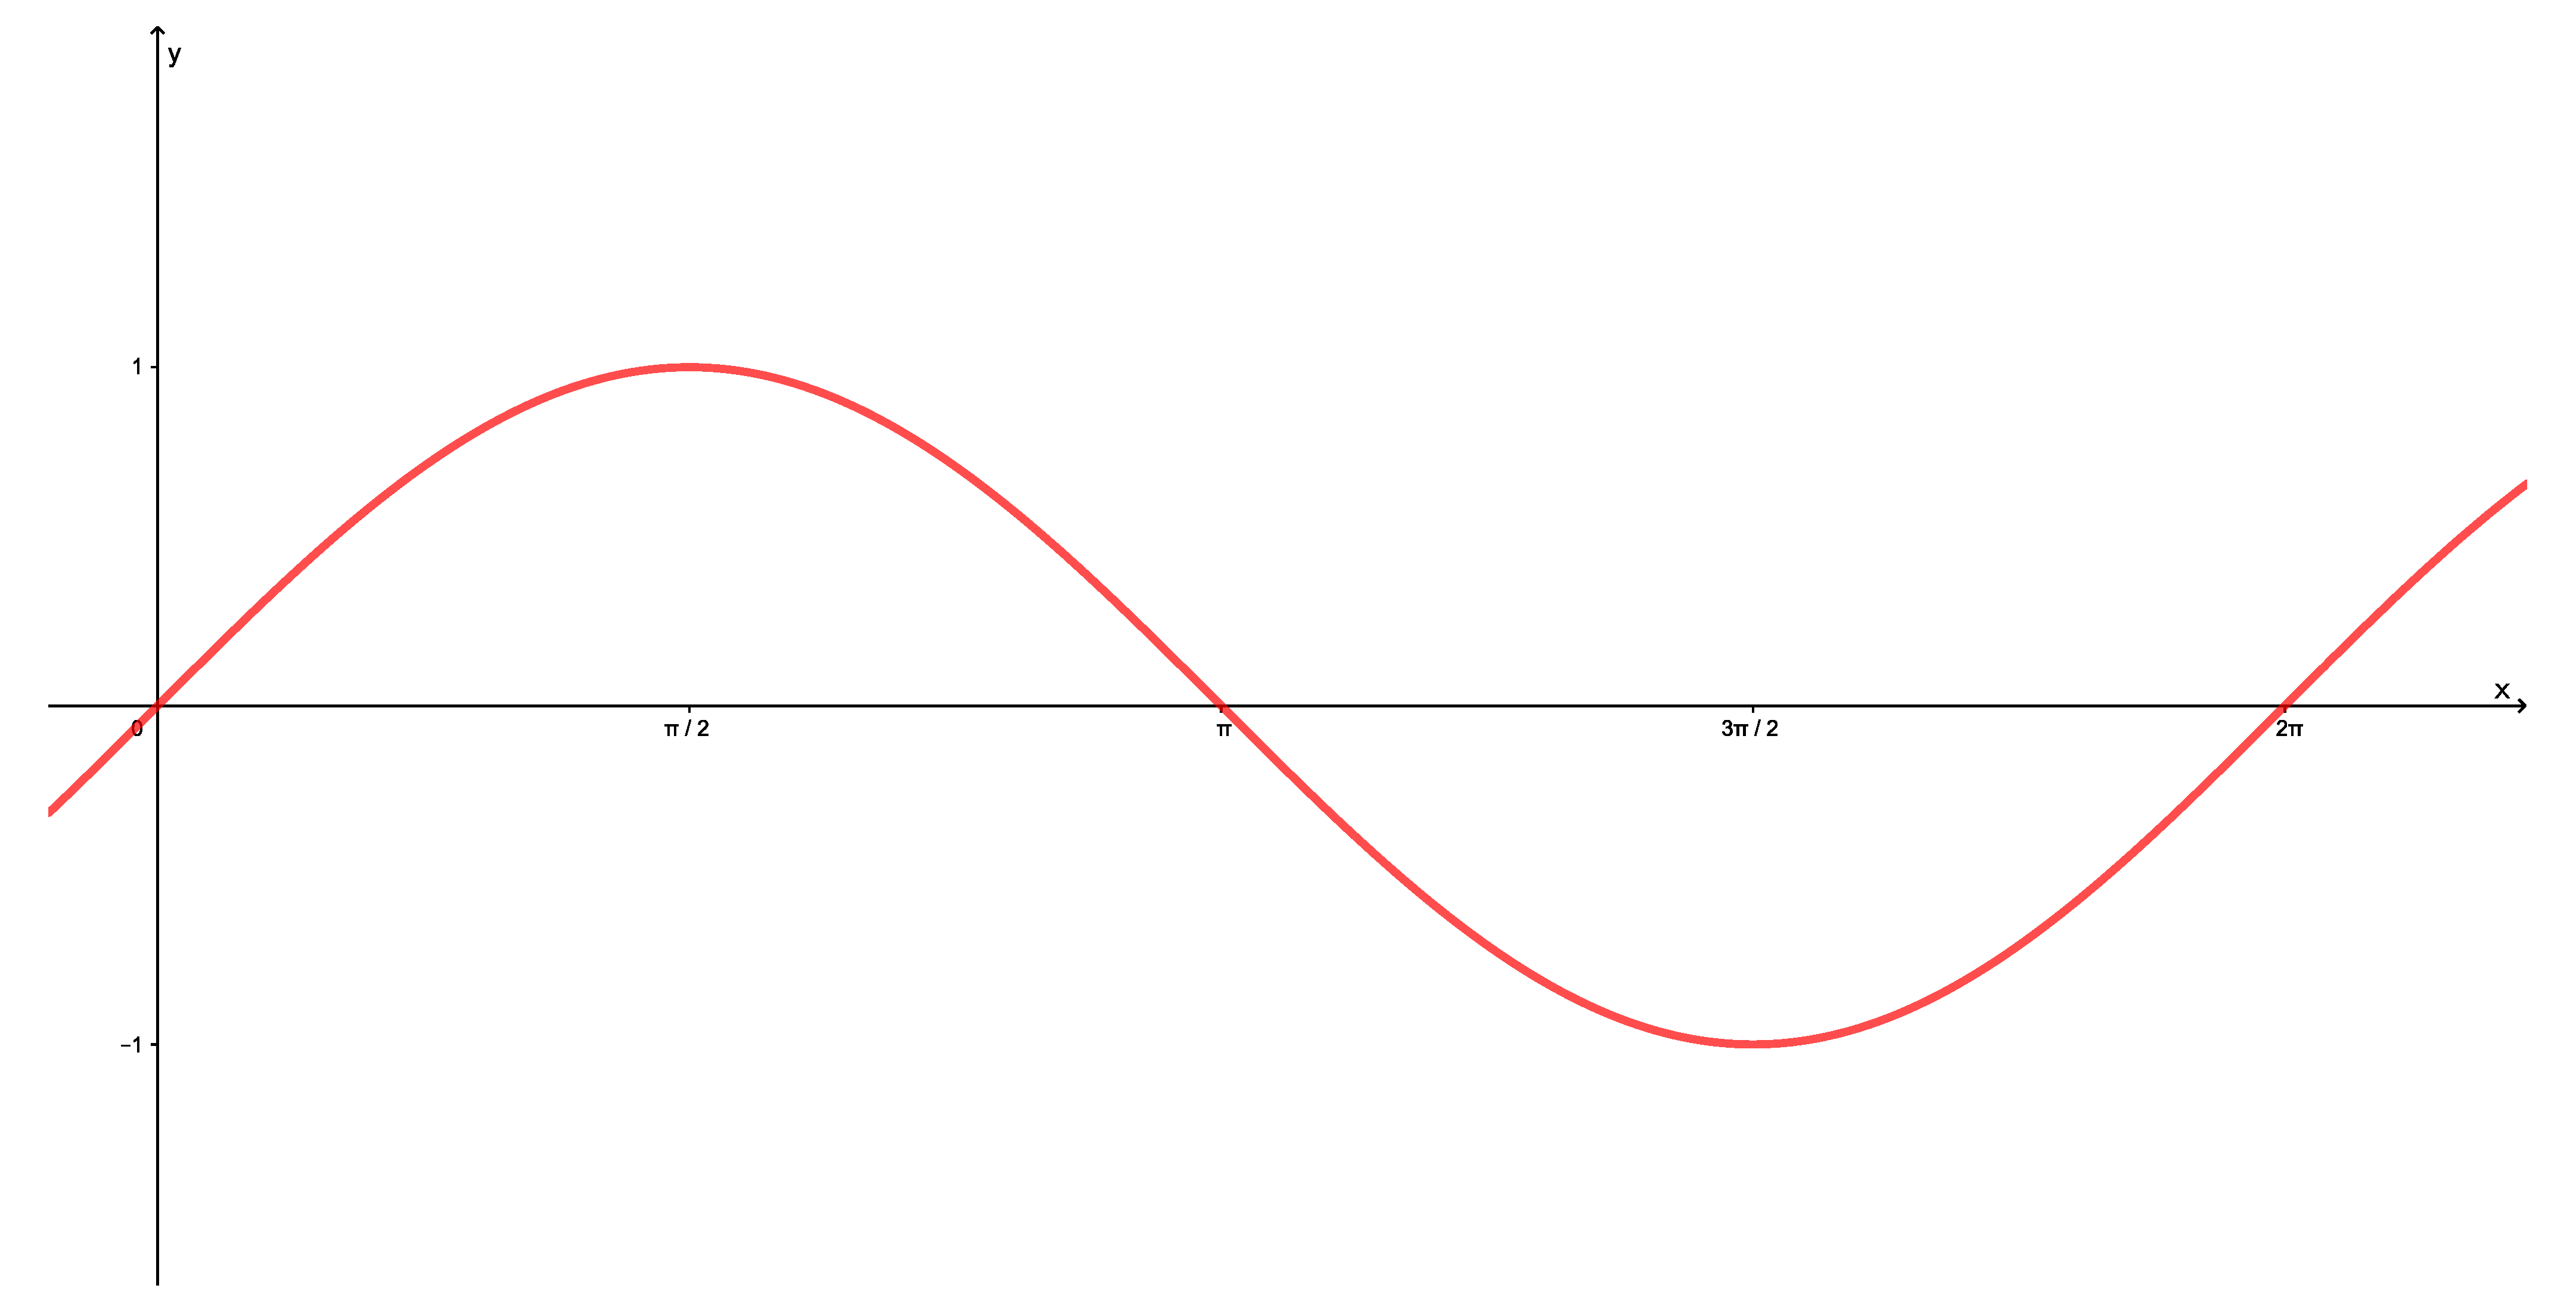
\includegraphics[scale=0.1]{Grap/sen}
\end{center}
\begin{center}
$y=\tan x$\\
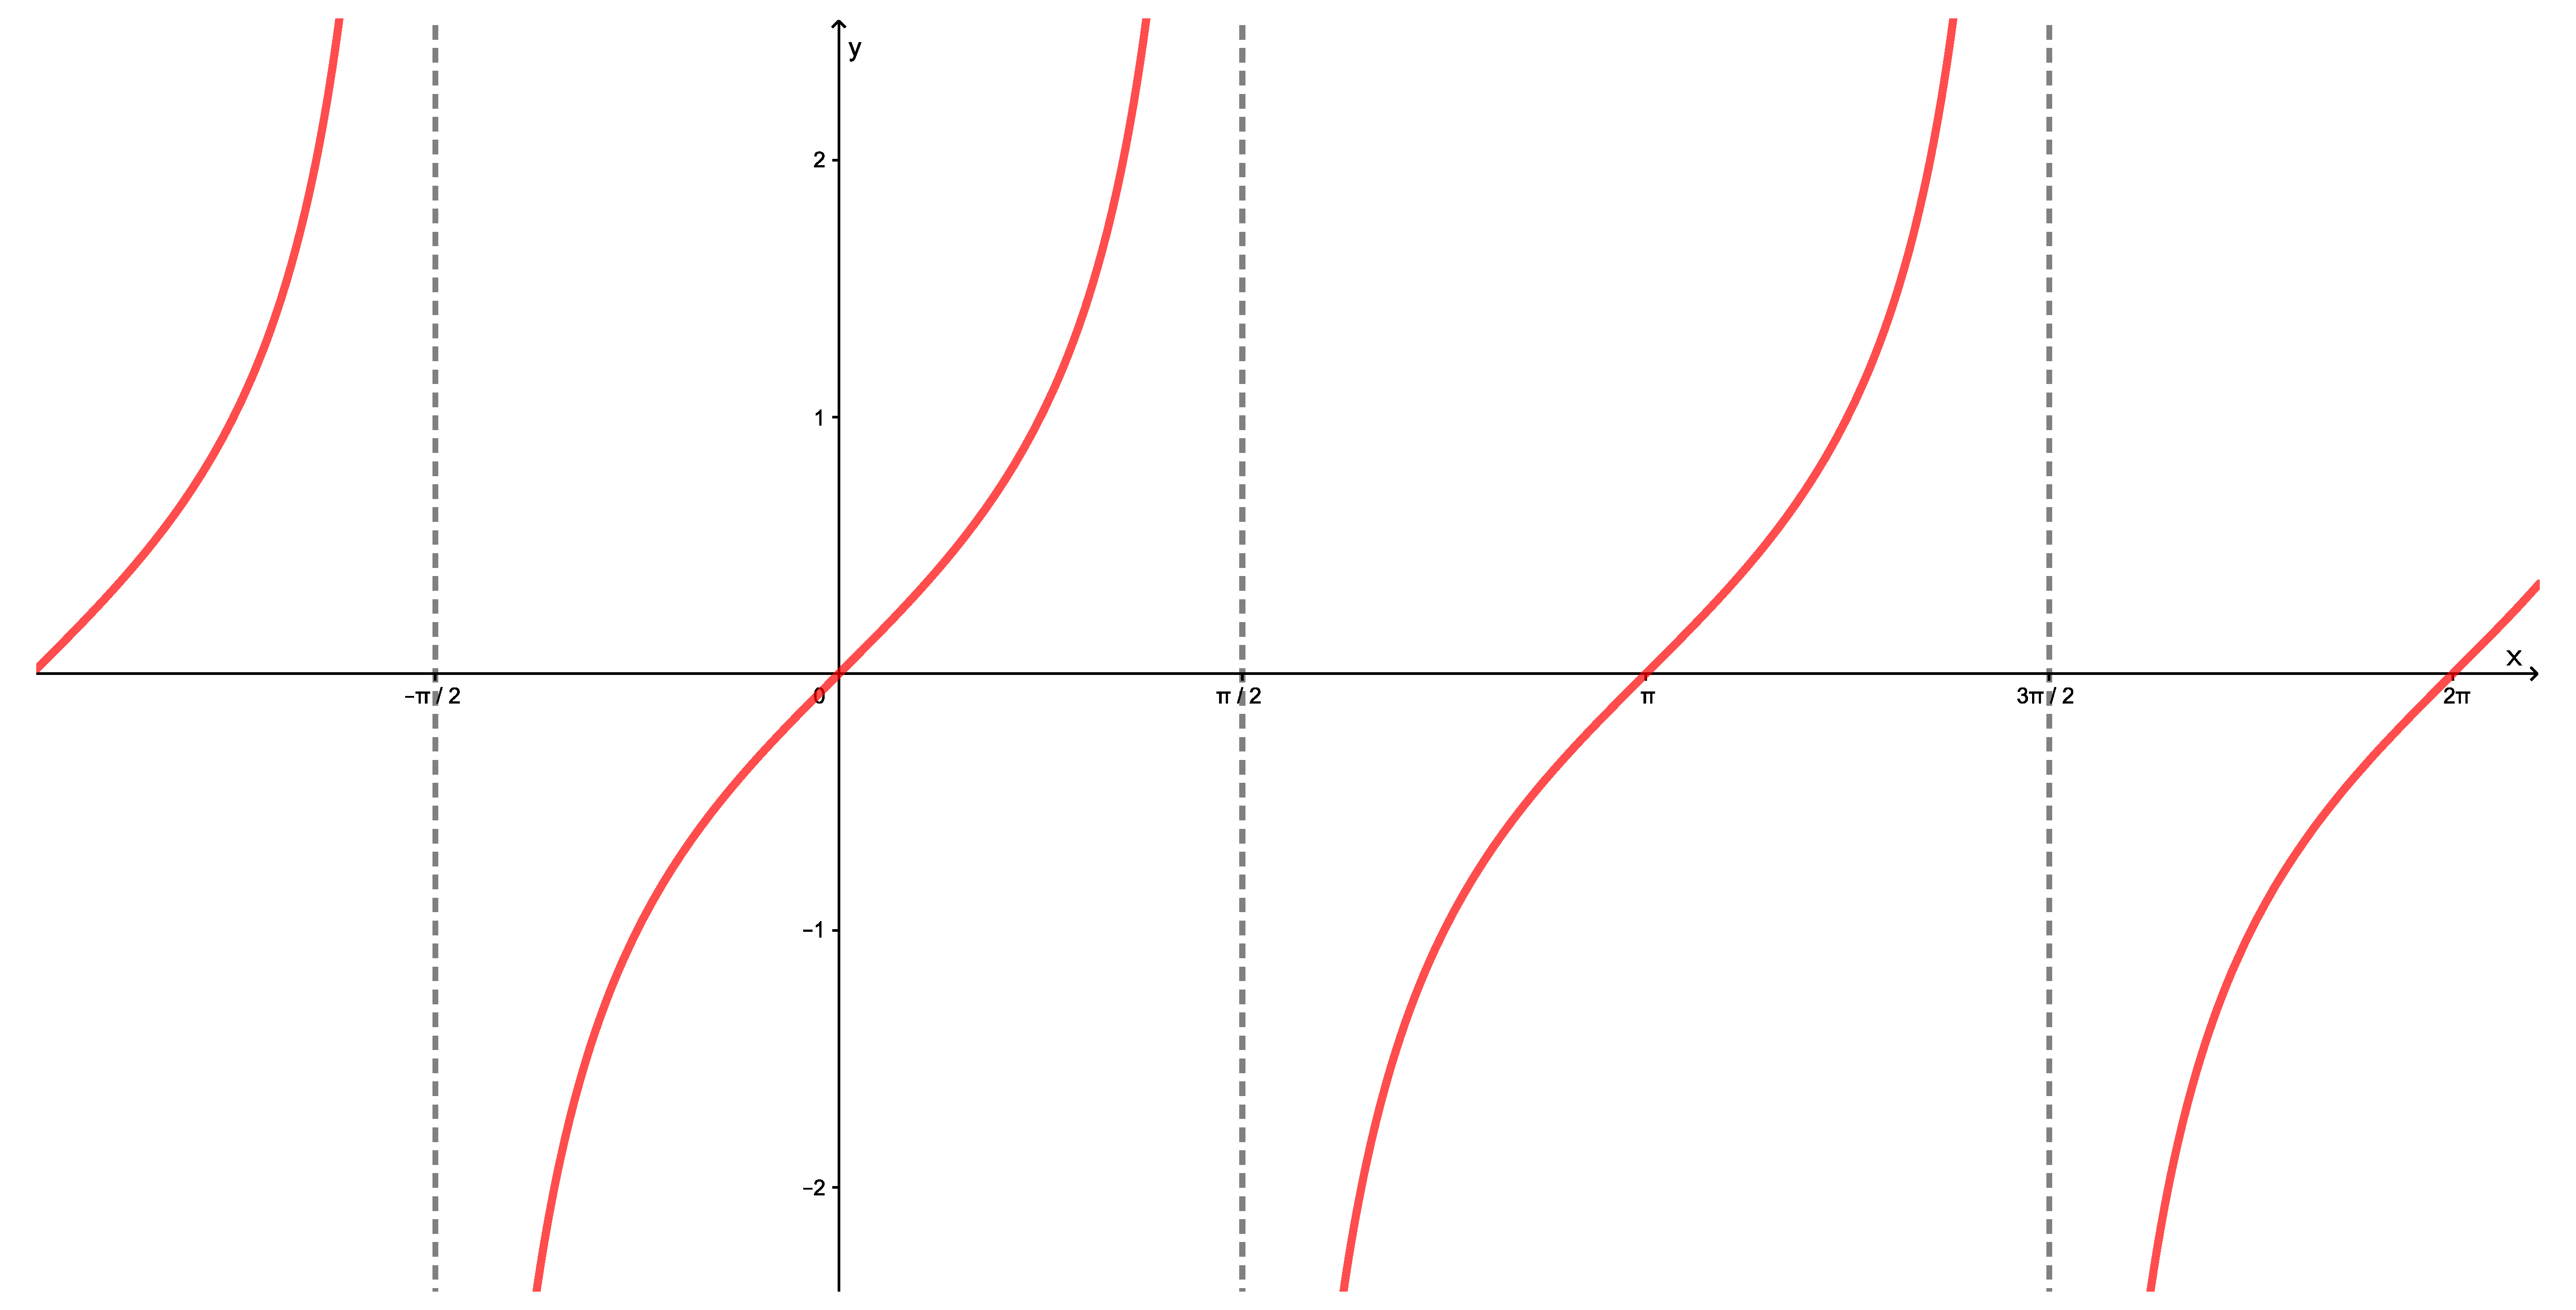
\includegraphics[scale=0.08]{Grap/tan}
\end{center}
\begin{center}
$y=\sec x$\\
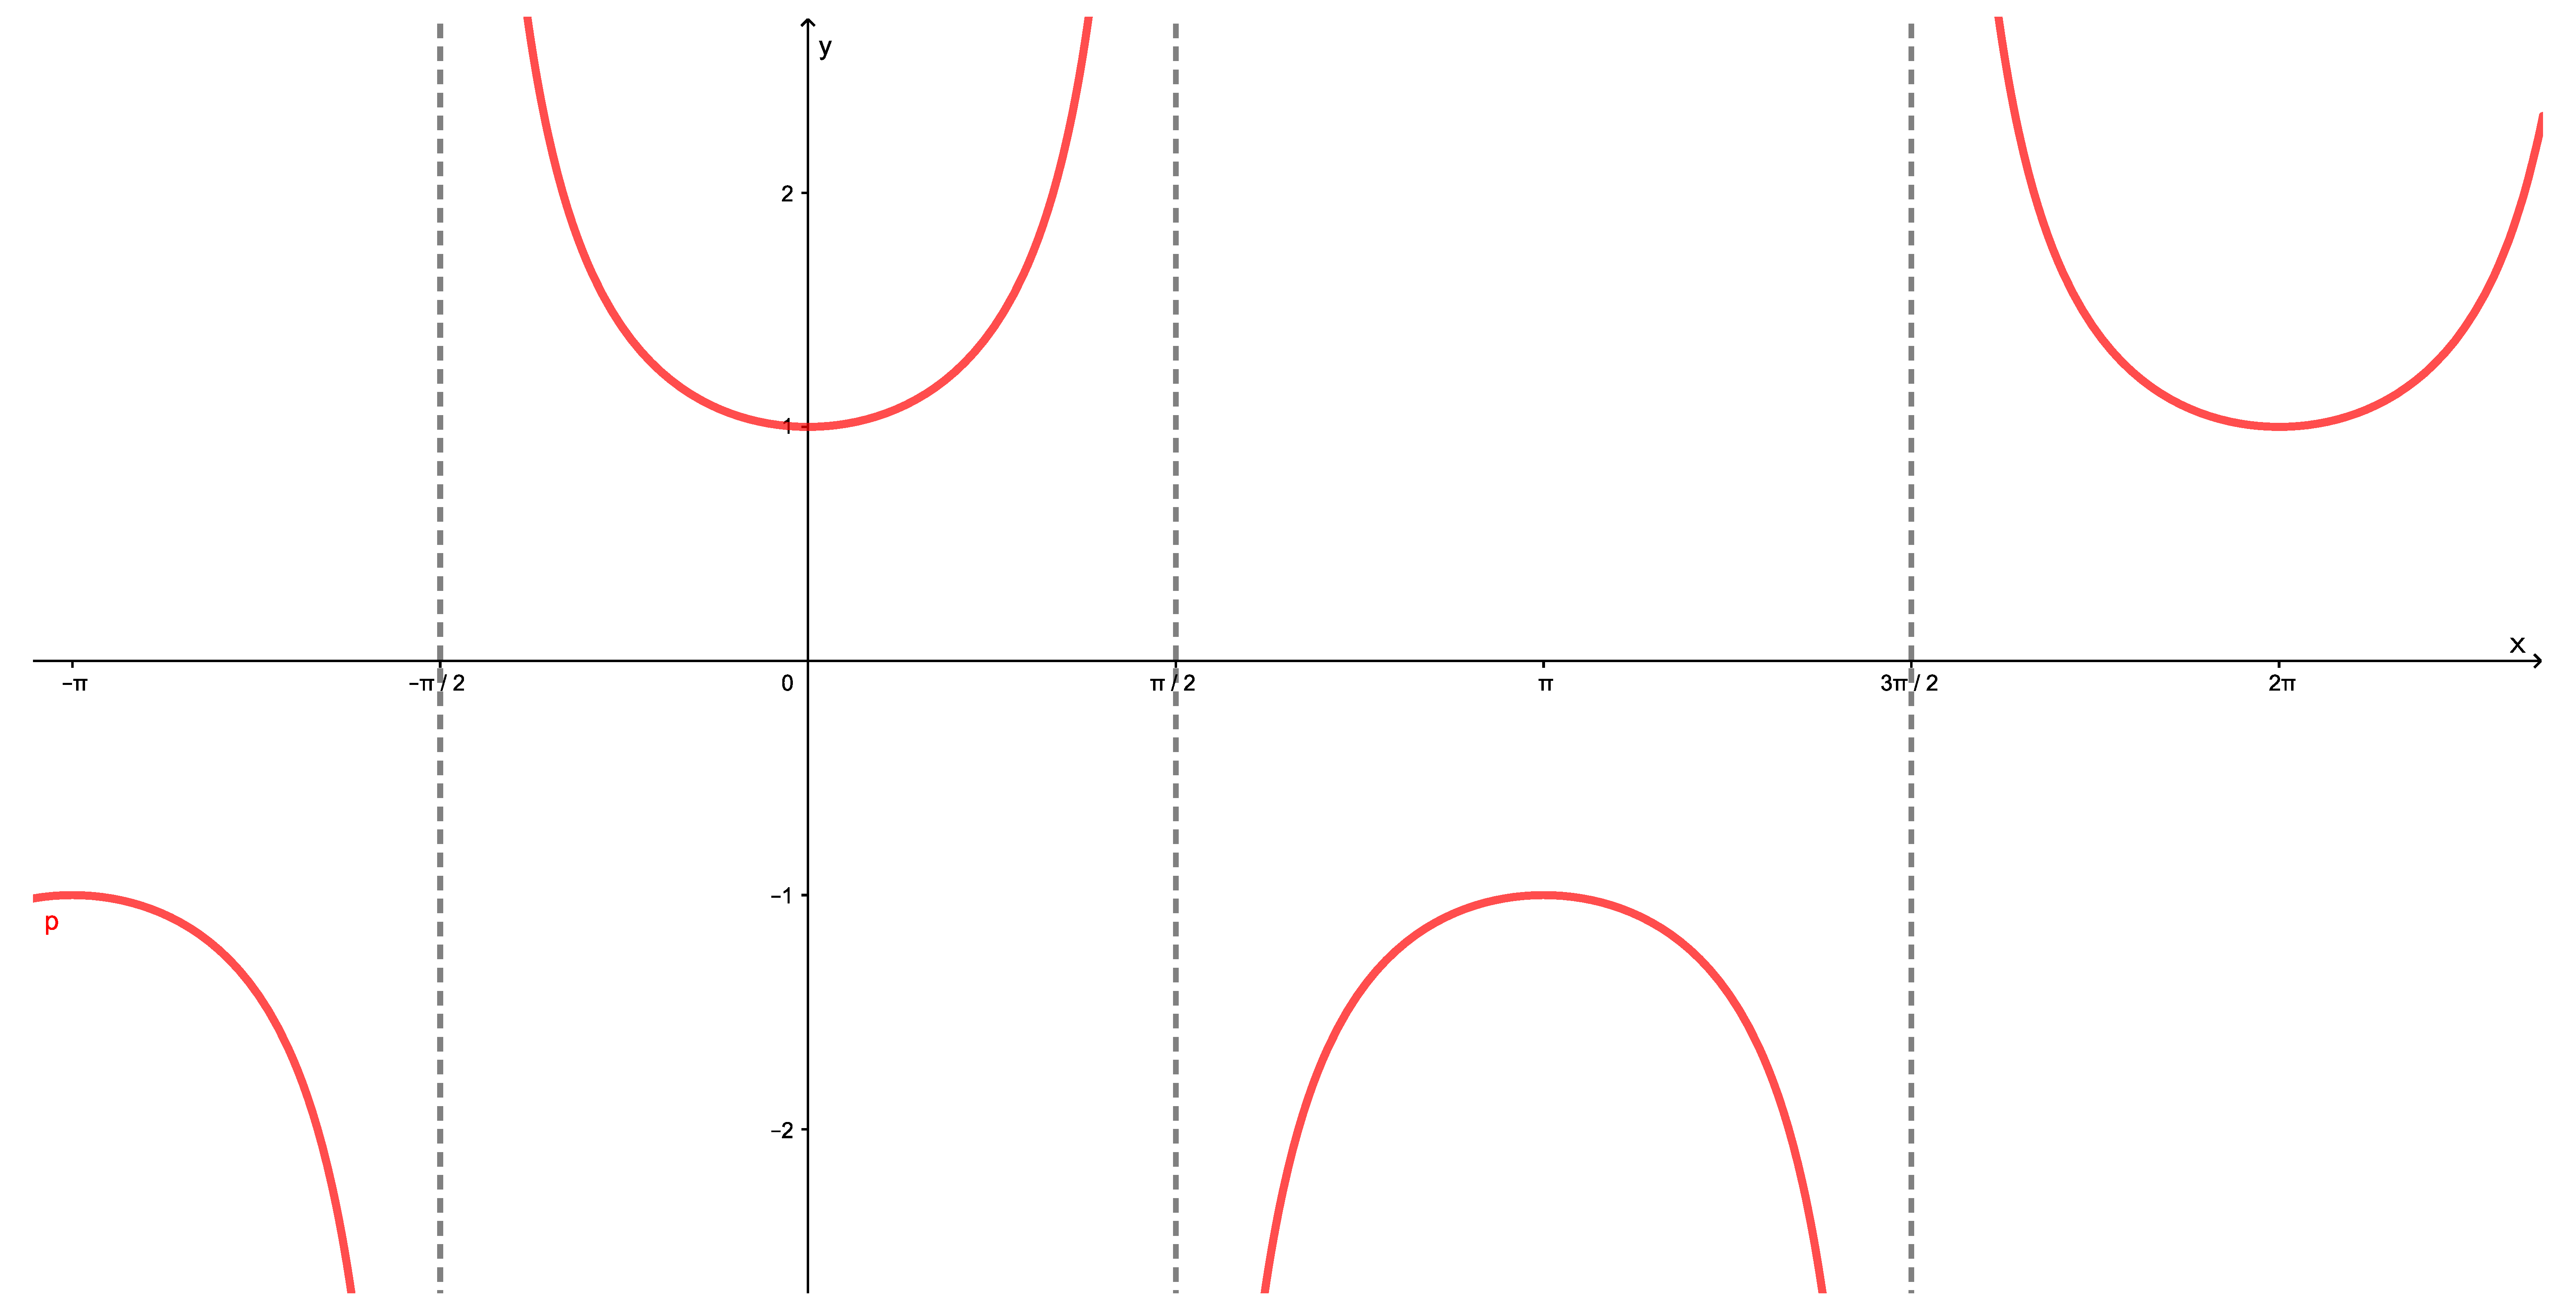
\includegraphics[scale=0.08]{Grap/sec}
\end{center}
\end{minipage} \begin{minipage}[c]{0.5\textwidth}
\begin{center} 
$y=\cos x$\\
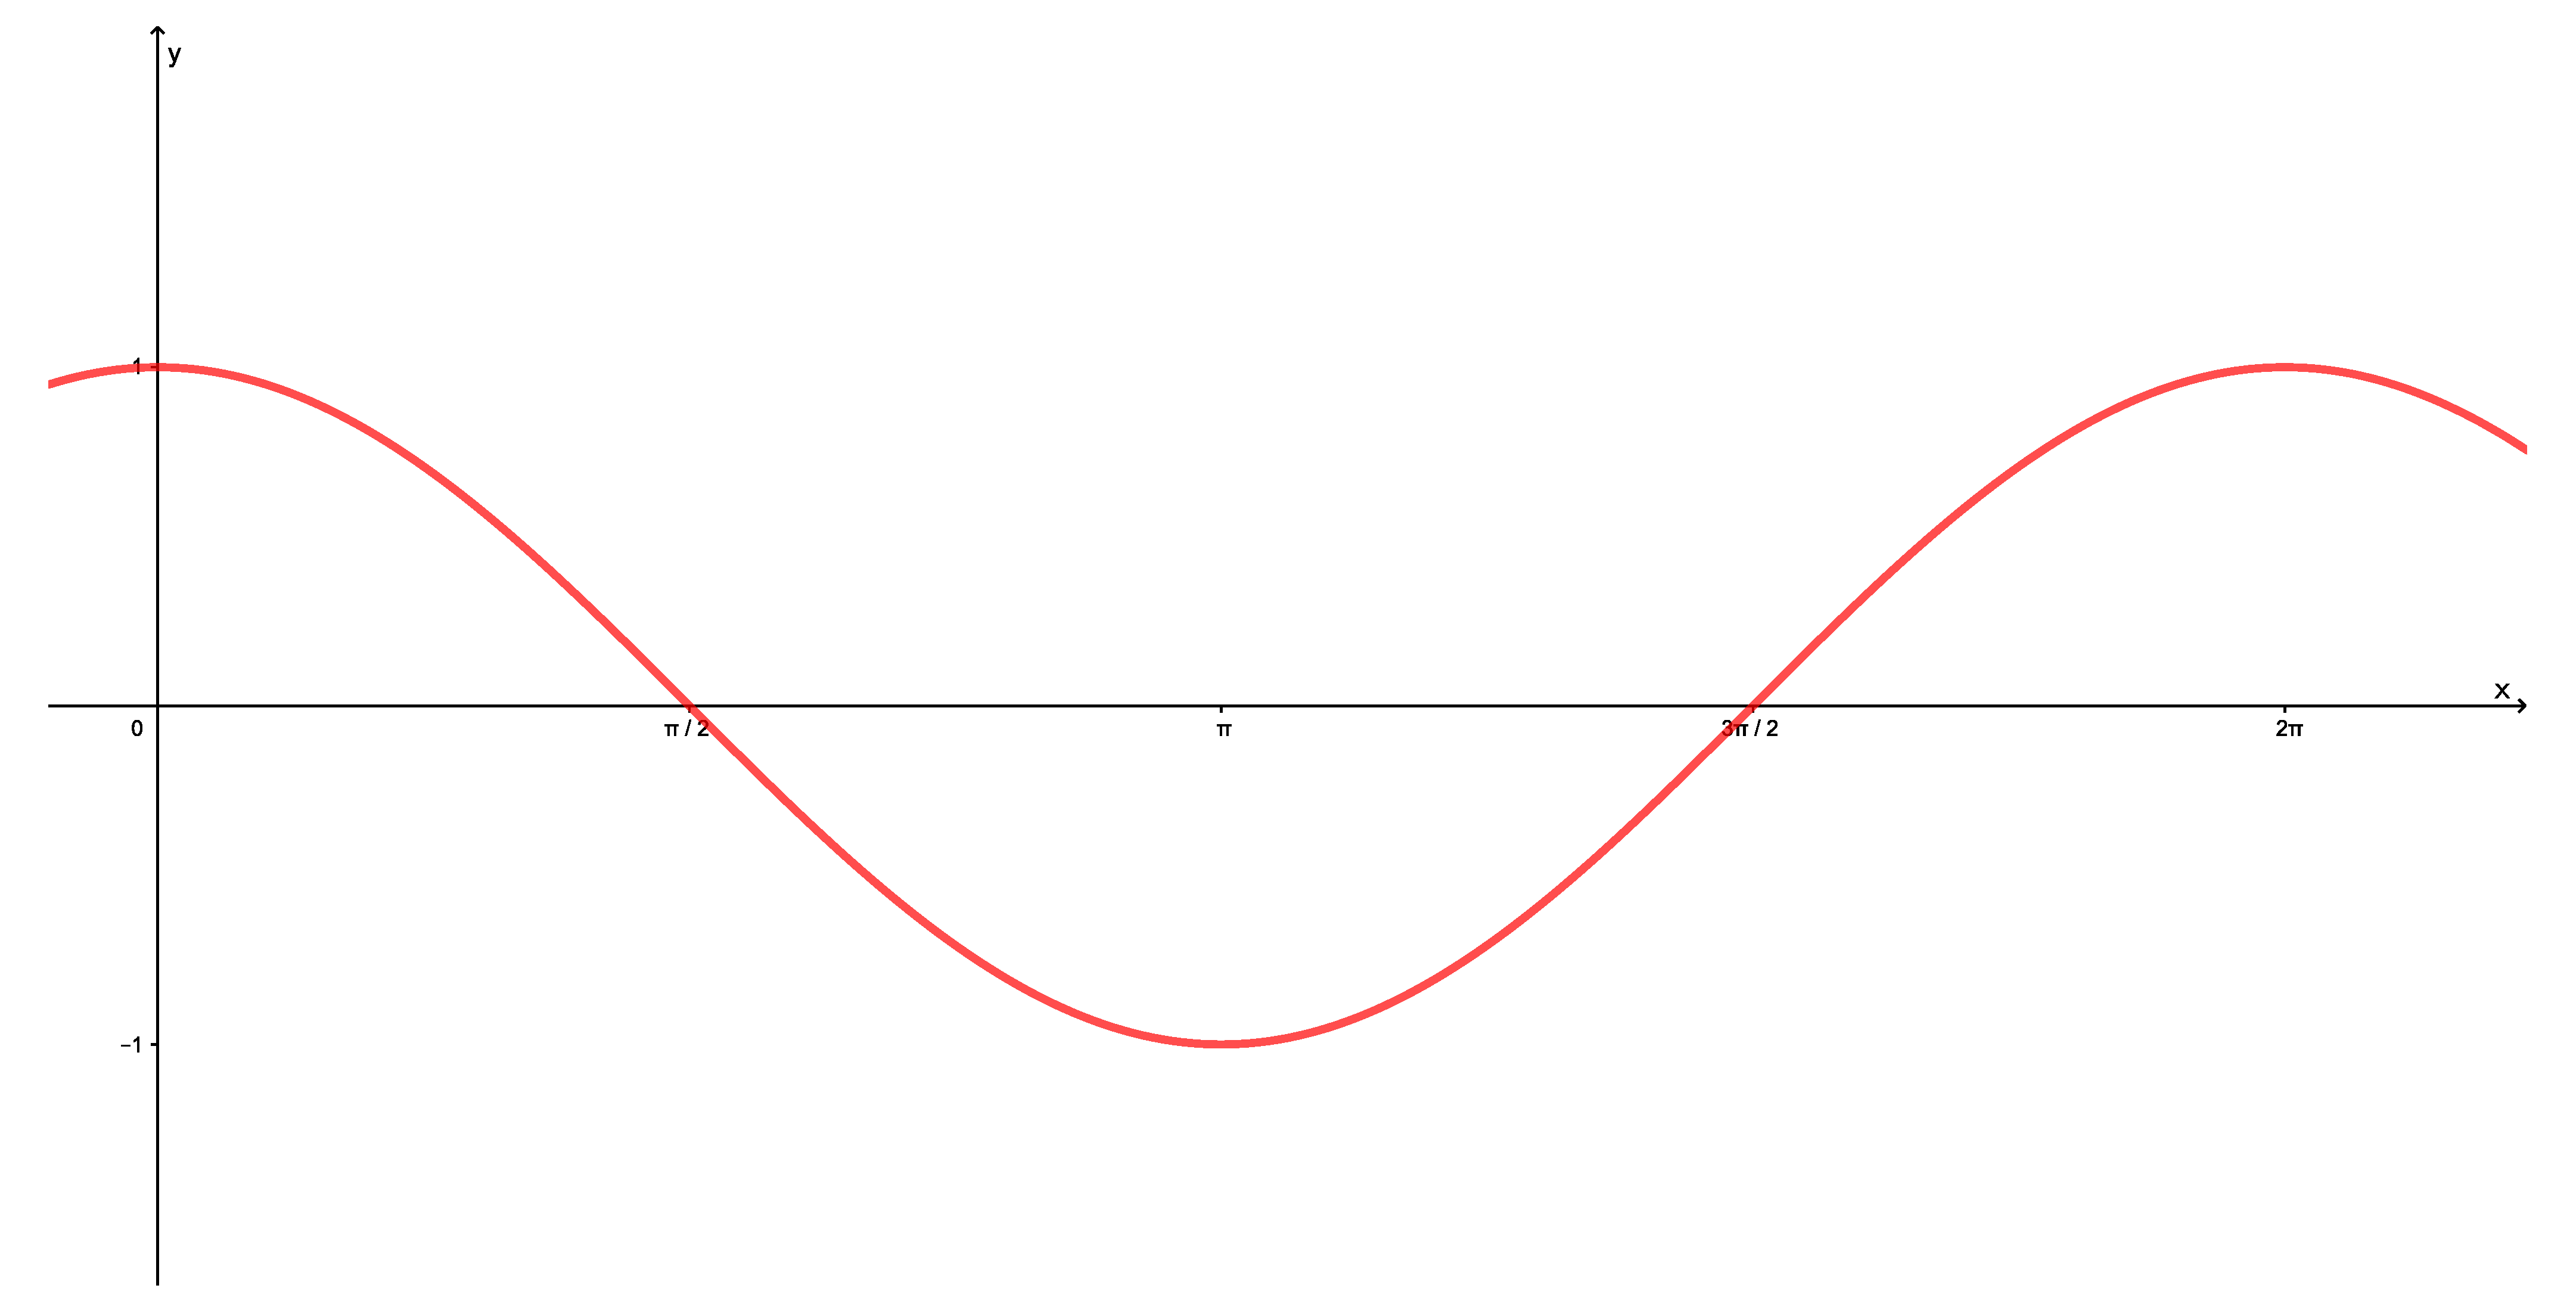
\includegraphics[scale=0.1]{Grap/cos}
\end{center}
\begin{center}
$y=\cot x$\\
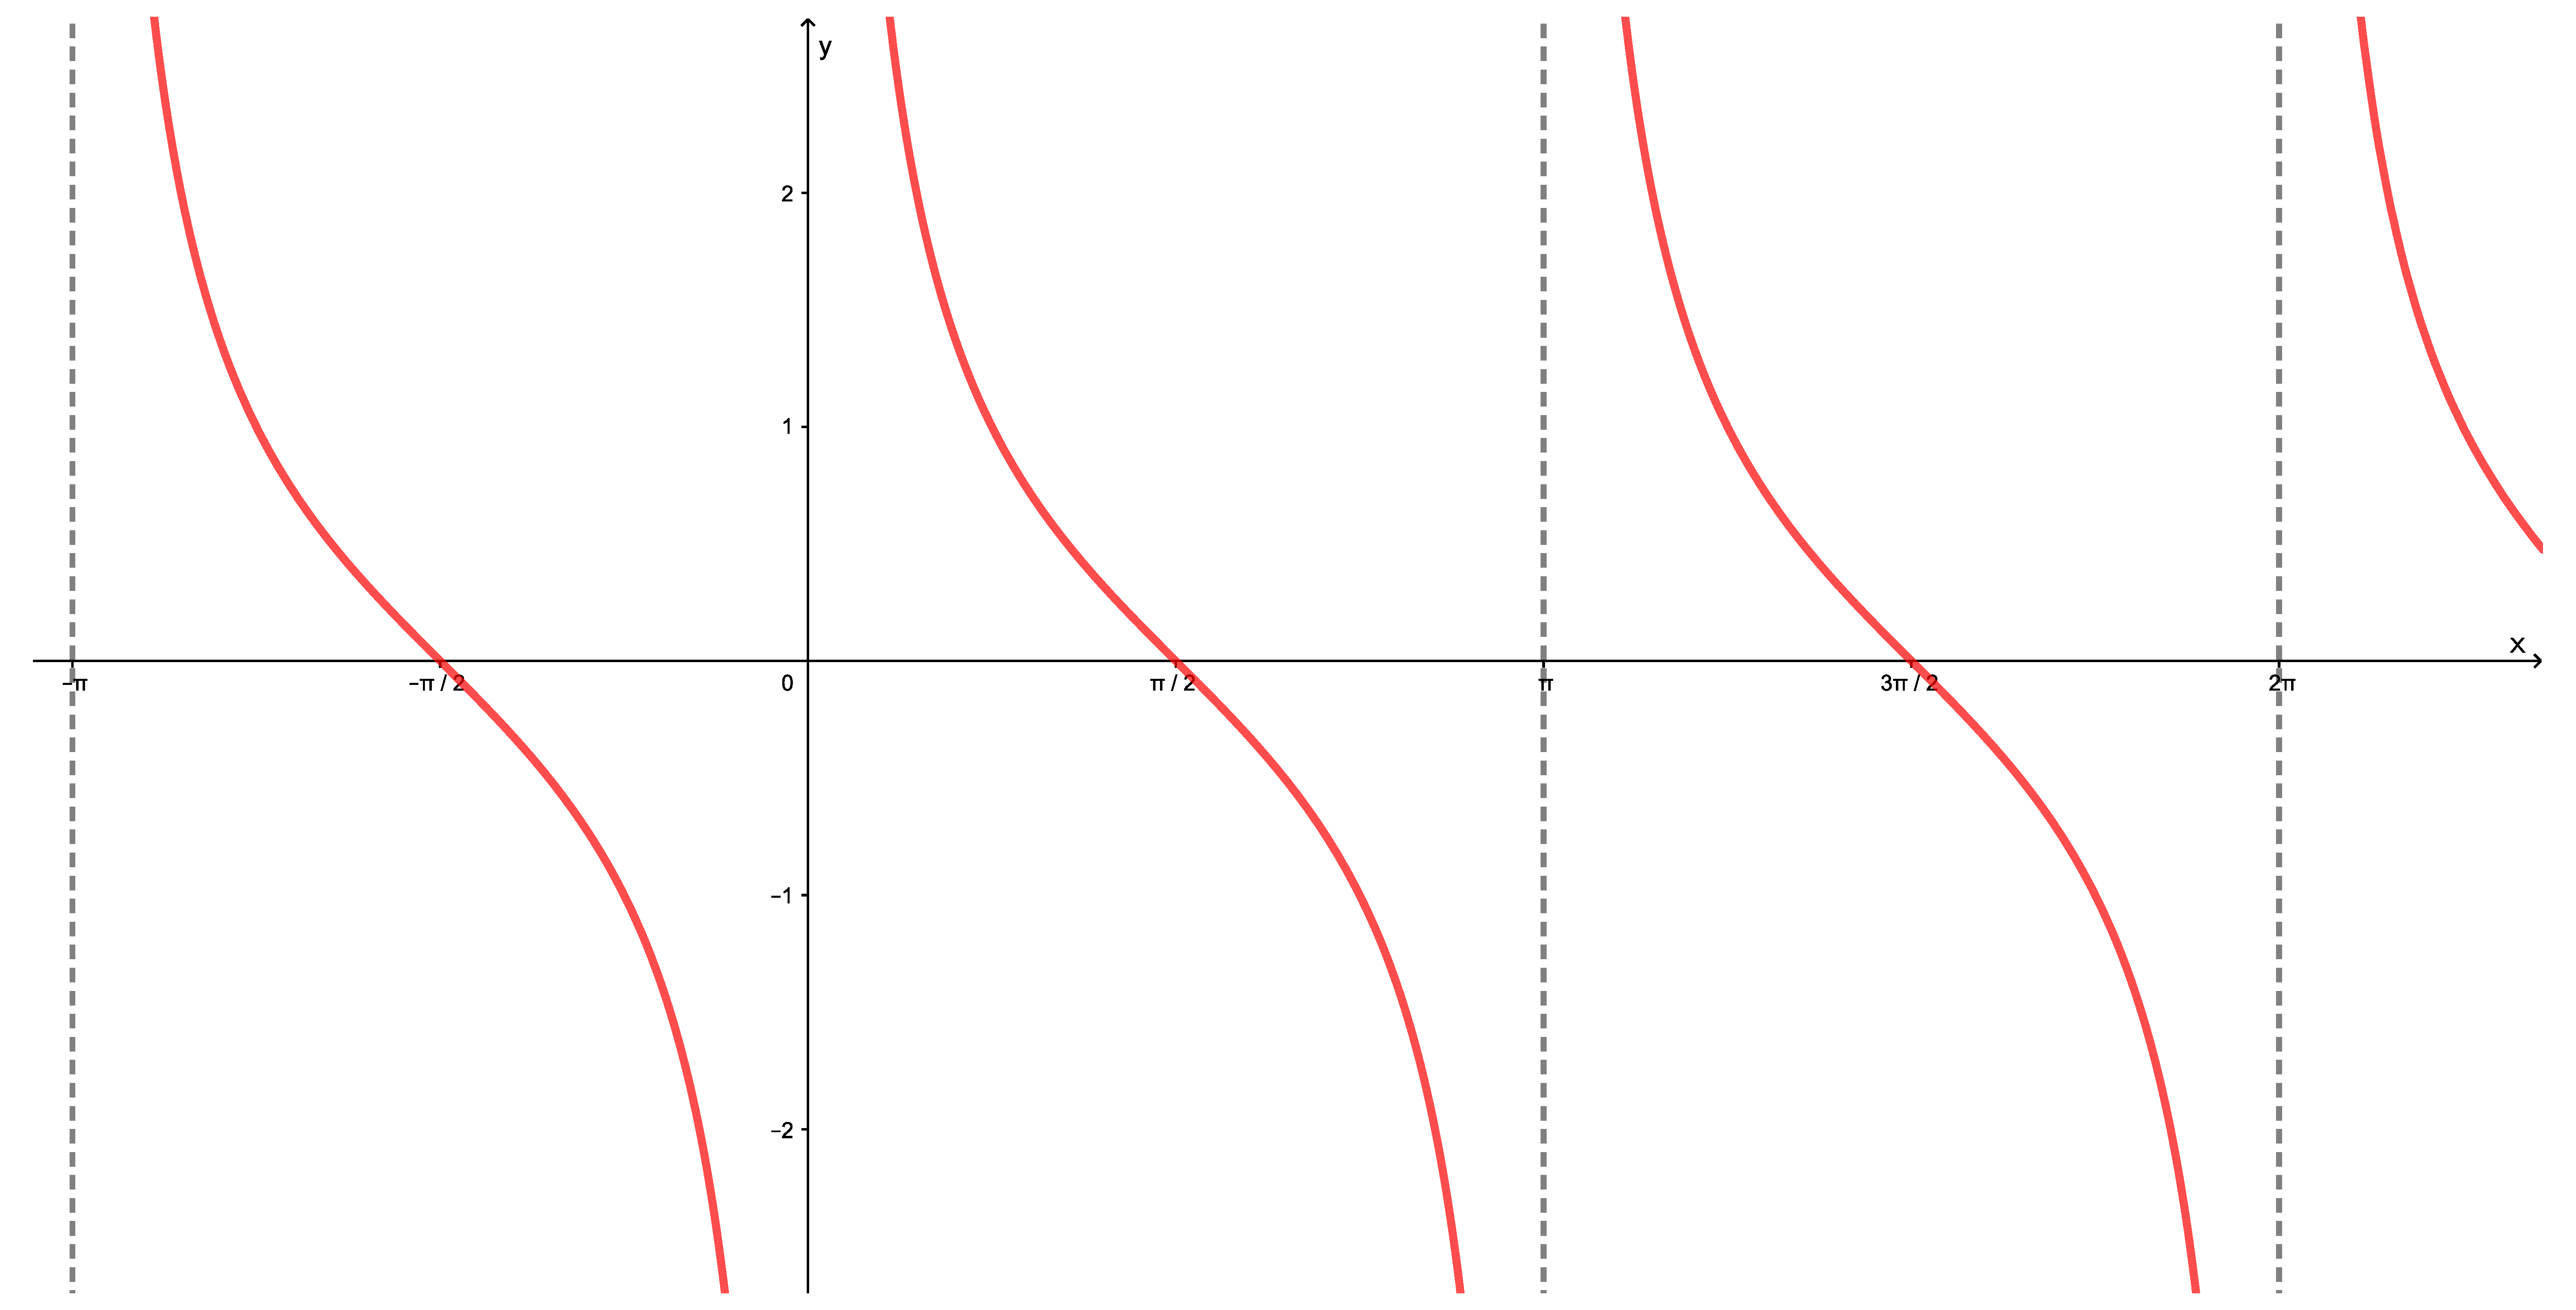
\includegraphics[scale=0.08]{Grap/cot}
\end{center}
\begin{center}
$y=\csc x$\\
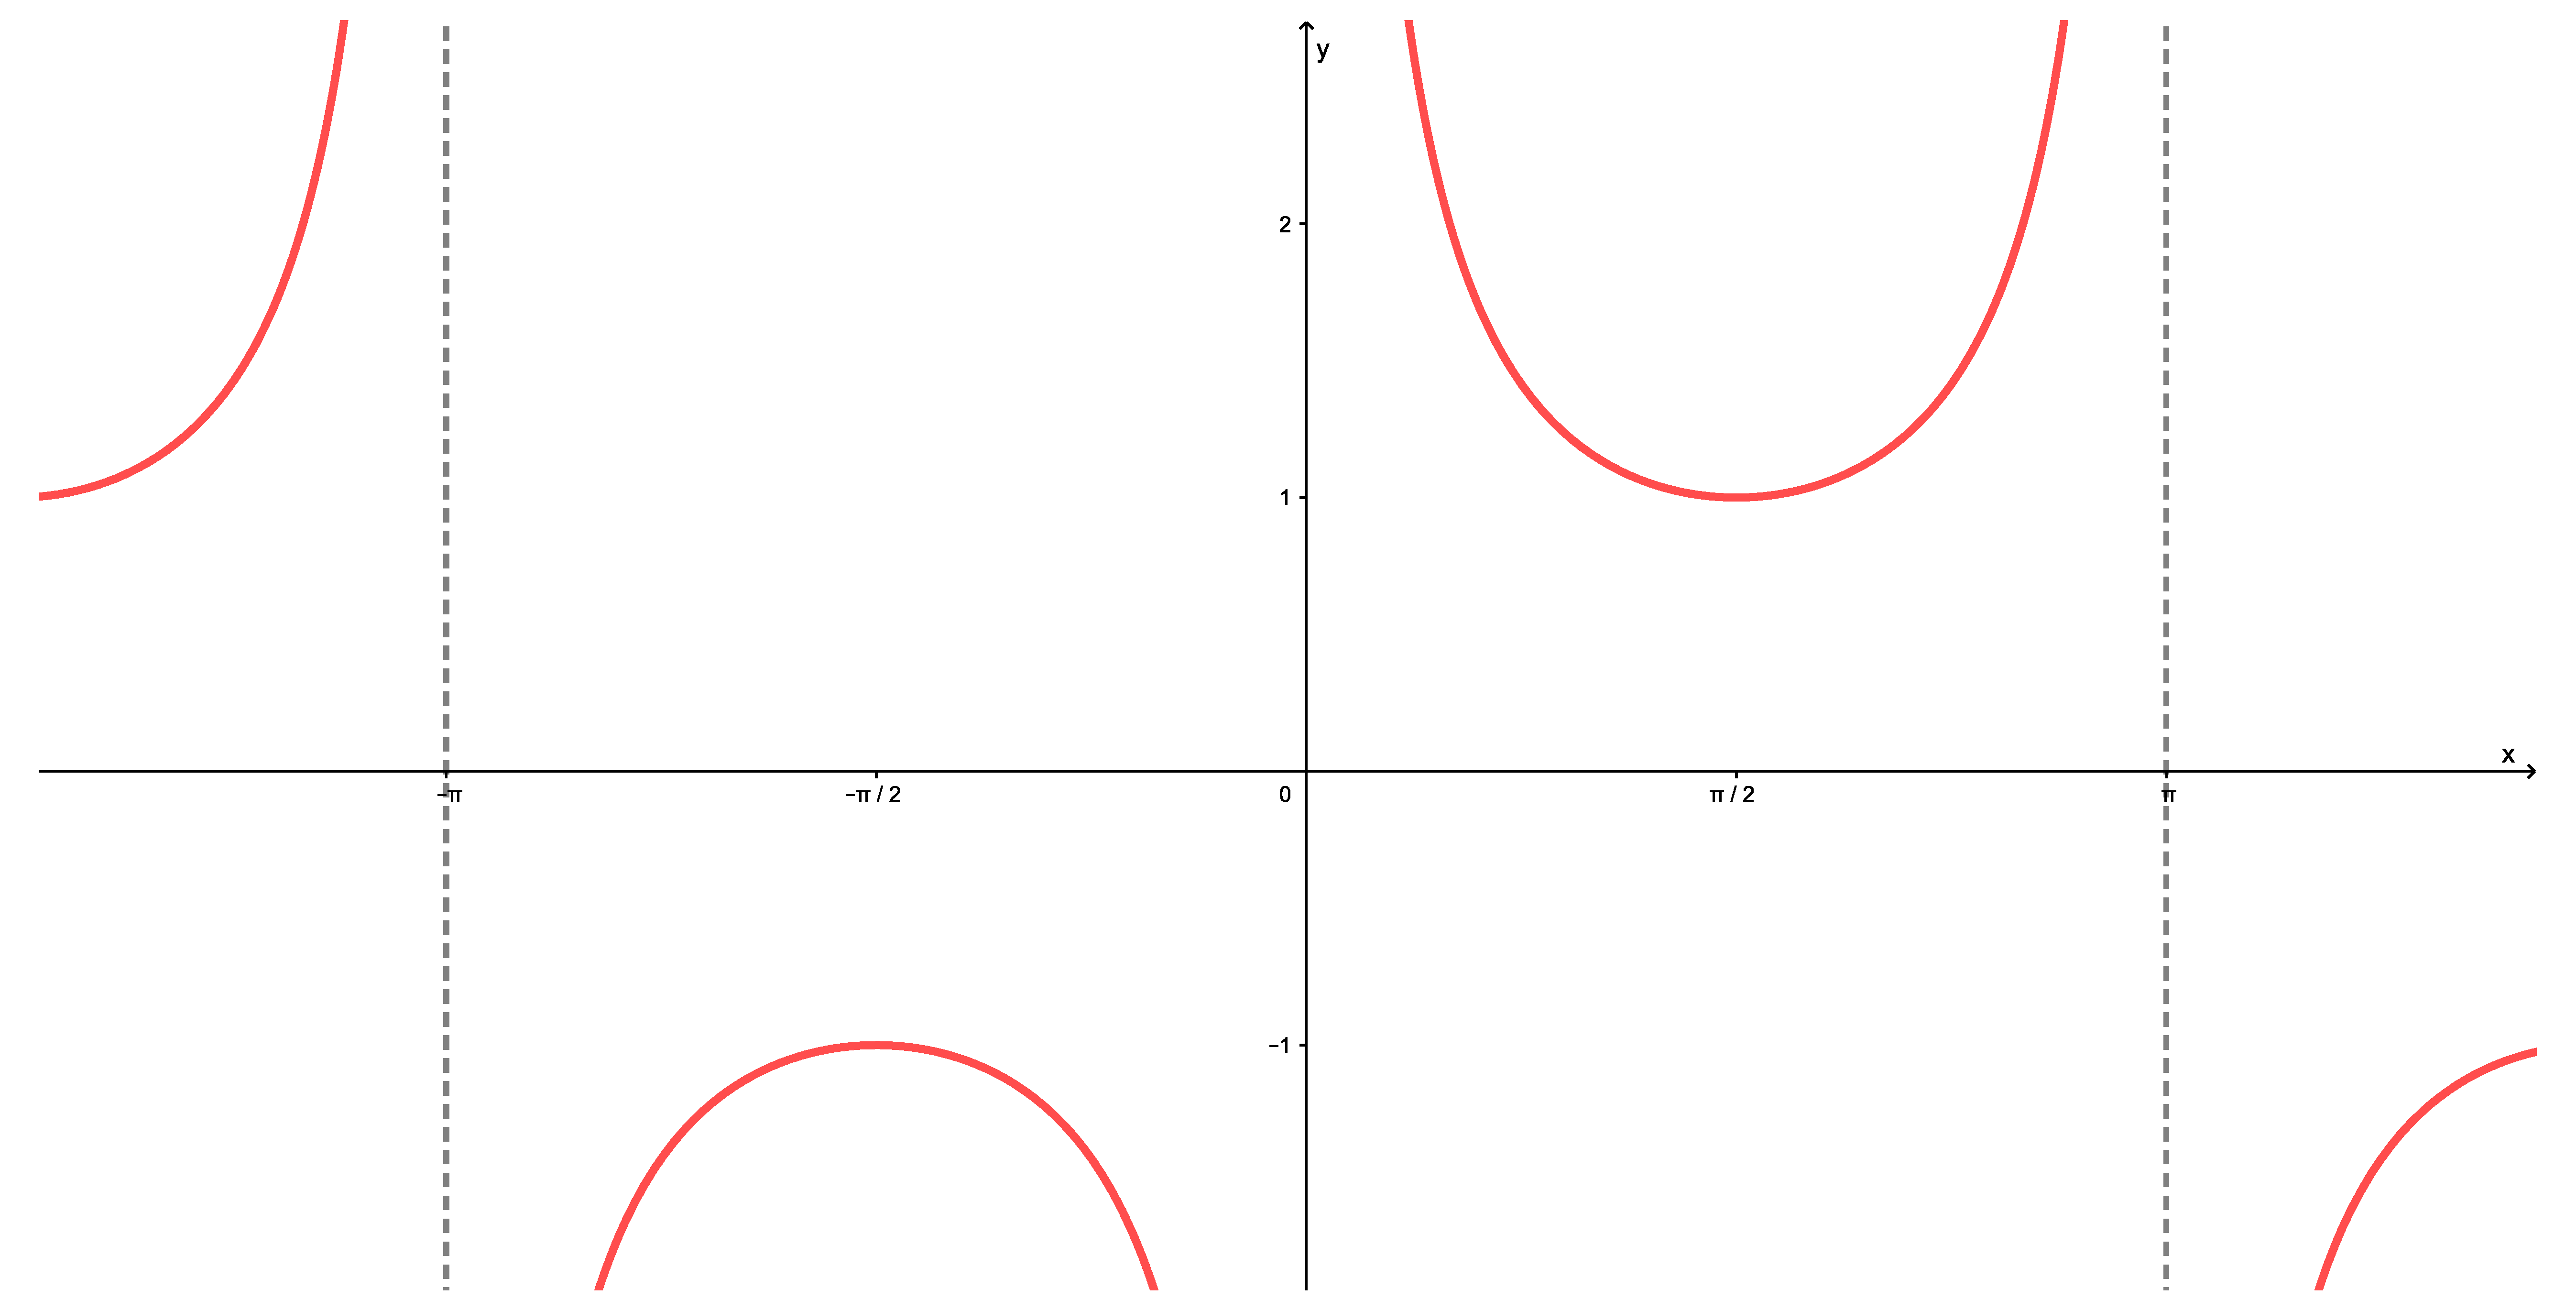
\includegraphics[scale=0.09]{Grap/csc}
\end{center}
\end{minipage}
\section*{Funciones de ángulos negativos}

\begin{minipage}[c]{0.3\textwidth}
$$ \sen (-A)=-\sen A$$

$$ \csc (-A)=-\csc A$$
\end{minipage}  \begin{minipage}[c]{0.3\textwidth}
$$\cos (-A)=\cos A$$

$$\sec (-A)=\sec A$$

\end{minipage}  \begin{minipage}[c]{0.3\textwidth}
$$\tan (-A)=-\tan A$$

$$\cot (-A)=-\cot A$$

\end{minipage}


\newpage

\section*{Formulas de adicion}
\begin{minipage}[c]{0.5\textwidth}
\begin{align*}
\sen (A \pm B) &= \sen A \cos B \pm \cos A \sen B\\\\
\cos (A \pm B) &= \cos A \cos B \mp \sen A \sen B
\end{align*}

\end{minipage} 
\begin{minipage}[c]{0.5\textwidth}
\begin{align*}
\tan (A \pm B) &= \frac{\tan A \pm \tan B}{1 \mp \tan A \tan B}\\\\
\cot (A \pm B) &= \frac{\cot A \cot B \mp 1}{\cot A \pm \cot B}
\end{align*}
\end{minipage}

\section*{Funciones de ángulos reducidos al primer cuadrante}
(con $k \in \mathbb{Z}$)
\begin{table}[htb]
\extrarowheight = -0.5ex
\renewcommand{\arraystretch}{1.71}
\centering
\begin{tabular}{|c|c|c|c|c|c|}
\hline
Función & $-A$ & $\frac{\pi}{2} \pm A$ & $\pi \pm A$ & $\frac{3\pi}{2} \pm A$ & $2k\pi + A$ \\ \hline
$\sen$ & $-\sen A$ & $\cos A$ & $\mp \sen A$ & $-\cos A$ & $\pm \sen A$ \\ \hline
$\cos$ & $\cos A$ & $\mp \sen A$ & $-\cos A$ & $\pm \sen A$ & $\cos A$ \\ \hline
$\tan$ & $-\tan A$ & $\mp \cot A$ & $\pm \tan A$ & $\mp \cot A$ & $\pm \tan A$ \\ \hline
$\csc$ & $-\csc A$ & $\sec A$ & $\mp \csc A$ & $-\sec A$ & $\pm \csc A$ \\ \hline
$\sec$ & $\sec A$ & $\mp \csc A$ & $-\sec A$ & $\pm \csc A$ & $\sec A$ \\ \hline
$\cot$ & $-\cot A$ & $\mp \tan A$ & $\pm \cot A$ & $\mp \tan A$ & $\pm \cot A$ \\ \hline
\end{tabular}
\end{table}

\section*{Relaciones entre funciones de los ángulos en el primer cuadrante}

\begin{table}[htb]
\extrarowheight = -0.5ex
\renewcommand{\arraystretch}{1.9}
\centering
\begin{tabular}{|c|c|c|c|c|c|c|}
\hline
Función & $\sen A = u$ & $\cos A = u $ & $\tan A = u$ & $\cot A = u$ & $\sec A = u$ & $\csc A = u$ \\ \hline
$\sen A$ & $u$ & $\sqrt{1-u^2}$ & $\frac{u}{\sqrt{1+u^2}}$ & $\frac{1}{\sqrt{1+u^2}}$ & $\frac{\sqrt{1-u^2}}{u}$ & $\frac{1}{u}$ \\ \hline
$\cos A$ & $\sqrt{1-u^2}$ & $u$ & $\frac{1}{\sqrt{1+u^2}}$ & $\frac{u}{\sqrt{1+u^2}}$ & $\frac{1}{u}$ & $\frac{\sqrt{1-u^2}}{u}$\\ \hline
$\tan A$ & $\frac{u}{\sqrt{1-u^2}}$ & $\frac{\sqrt{1-u^2}}{u}$ & $u$ & $\frac{1}{u}$ & $\sqrt{1-u^2}$ & $\frac{1}{\sqrt{1-u^2}}$\\ \hline
$\cot A$ & $\frac{\sqrt{1-u^2}}{u}$ & $\frac{u}{\sqrt{1-u^2}}$ & $\frac{1}{u}$ & $u$ & $\frac{1}{\sqrt{1-u^2}}$ & $\sqrt{1-u^2}$\\ \hline
$\sec A$ & $\frac{1}{\sqrt{1-u^2}}$ & $\frac{1}{u}$ & $\sqrt{1+u^2}$ & $\frac{\sqrt{1-u^2}}{u}$ & $u$ & $\frac{u}{\sqrt{1-u^2}}$\\ \hline
$\csc A$ & $\frac{1}{u}$ & $\frac{1}{\sqrt{1-u^2}}$ & $\frac{\sqrt{1+u^2}}{u}$ & $\sqrt{1+u^2}$ & $\frac{u}{\sqrt{1-u^2}}$ & $u$\\ \hline
\end{tabular}
\end{table}

\section*{Formulas del ángulo doble}
\begin{align*}
	\sen 2A &= 2\sen A \cos A \\[5pt]
	\cos 2A &= \cos^2 A -\sen^2 A = 1-2\sen^2 A = 2\cos^2 A - 1 \\
	\tan 2A &= \frac{2\tan A}{1-\tan^2 A}
\end{align*}

\section*{Formulas de medio ángulo}

\begin{align*}
	\sen \frac{A}{2} &= \pm\sqrt{\frac{1-\cos A}{2}}\,\,\, \begin{bmatrix}
+& \textrm{si} & A/2 & \textrm{esta} & \textrm{I\,o\,II\,\,cuadrante}\,\,\,\\ 
-& \textrm{si} & A/2 & \textrm{esta} & \textrm{III\,o\,IV\,\,cuadrante}\,\,\,\\ 
\end{bmatrix}\\
	\cos \frac{A}{2} &= \pm\sqrt{\frac{1+\cos A}{2}}\,\,\, \begin{bmatrix}
+& \textrm{si} & A/2 & \textrm{esta} & \textrm{I\,o\,IV\,\,cuadrante}\,\,\,\\ 
-& \textrm{si} & A/2 & \textrm{esta} & \textrm{II\,o\,III\,\,cuadrante}\,\,\,\\ 
\end{bmatrix}\\
	\tan \frac{A}{2} &= \pm\sqrt{\frac{1-\cos A}{1-\cos A}}\,\,\, \begin{bmatrix}
+& \textrm{si} & A/2 & \textrm{esta} & \textrm{I\,o\,III\,\,cuadrante}\,\,\,\\ 
-& \textrm{si} & A/2 & \textrm{esta} & \textrm{II\,o\,IV\,\,cuadrante}\,\,\,\\ 
\end{bmatrix}\\
&= \frac{\sen A}{1+\cos A} = \frac{1-\cos A}{\sen A} = \csc A - \cot A
\end{align*}

\section*{Formulas de ángulos múltiplos}

\begin{align*}
	\sen 3A &= 3\sen A - 4\sen^3 A \\[5pt]
	\cos 3A &= 4\cos^3 A - 3\cos A  \\
	\tan 3A &= \frac{3\tan A-\tan^3 A}{1-3\tan^2 A}\\
	\sen 4A &= 4\sen A \cos A - 8 \sen^3 A \cos A \\[5pt]
	\cos 4A &= 8\cos^4 A - 8\cos^2 A + 1 \\
	\tan 4A &= \frac{4\tan A - 4\tan^3 A}{1-6\tan^2 A + \tan^4 A}\\
	\sen 5A &= 5\sen A - 20\sen^3 A +16\sen^5 A\\[5pt]
	\cos 5A &= 16\cos^3 A - 20\cos^3 A +5\cos A \\
	\tan 5A &= \frac{\tan^5 A - 10\tan^3 A + 5\tan A}{1-10\tan^2 A + 5\tan^4 A}
\end{align*}

\section*{Potencias de funciones trigonométricas}

\begin{minipage}[c]{0.5\textwidth}
\begin{align*}
\sen^2 A &= \frac{1}{2}- \frac{1}{2} \cos 2A\\
\cos^2 A &= \frac{1}{2}+ \frac{1}{2} \cos 2A\\
\sen^3 A &= \frac{3}{4}\sen A- \frac{1}{4} \sen 3A\\
\cos^3 A &= \frac{3}{4}\cos A+ \frac{1}{4} \cos 3A
\end{align*}

\end{minipage} 
\begin{minipage}[c]{0.5\textwidth}
\begin{align*}
\sen^4 A &= \frac{3}{8}- \frac{1}{2} \cos 2A + \frac{1}{8}\cos 4A\\
\cos^4 A &= \frac{3}{8}+ \frac{1}{2} \cos 2A + \frac{1}{8}\cos 4A\\
\sen^5 A &= \frac{5}{8}\sen A- \frac{5}{16} \sen 3A + \frac{1}{16}\sen 5A\\
\cos^5 A &= \frac{5}{8}\cos A+ \frac{5}{16} \cos 3A + \frac{1}{16}\cos 5A
\end{align*}
\end{minipage}

\section*{Suma, diferencia y producto de las funciones}

\begin{align*}
\sen A + \sen B &= 2\sen\left( \frac{A+B}{2} \right)\cos\left( \frac{A-B}{2}\right)\\
\sen A - \sen B &= 2\cos\left( \frac{A+B}{2} \right)\sen\left( \frac{A-B}{2}\right)\\
\cos A + \cos B &= 2\cos\left( \frac{A+B}{2} \right)\cos\left( \frac{A-B}{2}\right)\\
\cos A - \cos B &= 2\sen\left( \frac{A+B}{2} \right)\sen\left( \frac{A-B}{2}\right)\\
\sen A \sen B &= \frac{1}{2}\left[ \cos (A-B)-\cos (A+B) \right]\\
\cos A \cos B &= \frac{1}{2}\left[ \cos (A-B)+\cos (A+B) \right]\\
\sen A \cos B &= \frac{1}{2}\left[ \sen (A-B)+\sen (A+B) \right]\\
\cos A \sen B &= \frac{1}{2}\left[ \sen (A+B)-\sen (A-B) \right]
\end{align*}

\section*{Formulas generales}

\begin{align*}
&\sen nA = \sen A \left[  (2\cos A)^{n-1}-\begin{pmatrix}n-2 \\1\end{pmatrix} (2\cos A)^{n-3}+\begin{pmatrix}n-3 \\1\end{pmatrix}(2\cos A)^{n-5} - \cdot \cdot \cdot  \right]\\\\
&\cos nA = \frac{1}{2} \left[  (2\cos A)^{n}- n (2\cos A)^{n-2}+\frac{n}{2}\begin{pmatrix}n-3 \\1\end{pmatrix}(2\cos A)^{n-4} - \frac{n}{3}\begin{pmatrix}n-4 \\2\end{pmatrix}(2\cos A)^{n-6} +\cdot \cdot \cdot  \right]\\\\
&\sen^{2n-1} A = \frac{(-1)^{n-1}}{2^{2n-2}} \left[ \sen (2n-1)A - \begin{pmatrix}2n-2 \\1\end{pmatrix}\sen (2n-3)A+\cdot \cdot \cdot (-1)^{n-1}\begin{pmatrix}2n-1 \\n-1\end{pmatrix}\sen A \right] \\\\
&\cos^{2n-1} A = \frac{1}{2^{2n-2}} \left[ \cos (2n-1)A + \begin{pmatrix}2n-2 \\1\end{pmatrix}\cos (2n-3)A+\cdot \cdot \cdot +\begin{pmatrix}2n-1 \\n-1\end{pmatrix}\cos A \right] \\\\
&\sen^{2n} A = \frac{1}{2^{2n}}\begin{pmatrix}2n \\n\end{pmatrix}+\frac{(-1)^{n}}{2^{2n-1}}\left[ \cos 2nA - \begin{pmatrix}2n \\1\end{pmatrix}\cos (2n-2)A + \cdot \cdot \cdot (-1)^{n-1}\begin{pmatrix}2n \\n-1\end{pmatrix} \cos 2A \right]\\\\
&\cos^{2n} A = \frac{1}{2^{2n}}\begin{pmatrix}2n \\n\end{pmatrix}+\frac{1}{2^{2n-1}}\left[ \cos 2nA + \begin{pmatrix}2n \\1\end{pmatrix}\cos (2n-2)A + \cdot \cdot \cdot +\begin{pmatrix}2n \\n-1\end{pmatrix} \cos 2A \right]
\end{align*}

\clearpage

\section*{Funciones trigonométricas inversas}

\begin{table}[htb]
\extrarowheight = -0.5ex
\renewcommand{\arraystretch}{1.9}
\centering
\begin{tabular}{|c|c|}
\hline
Valores principales para $x \geq  0$ & Valores principales para $x<0$\\ \hline
$0\leq \sen^{-1} x  \leq \frac{\pi}{2}$ &  $-\frac{\pi}{2} \leq \sen^{-1} x < 0$\\ \hline
$0\leq \cos^{-1} x  \leq \frac{\pi}{2}$ &  $\frac{\pi}{2} < \cos^{-1} x \leq \pi$\\ \hline
$0\leq \tan^{-1} x  < \frac{\pi}{2}$ &  $-\frac{\pi}{2} < \tan^{-1} x < 0$\\ \hline
$0\leq \cot^{-1} x  \leq \frac{\pi}{2}$ &  $\frac{\pi}{2} < \cot^{-1} x < \pi$\\ \hline
$0\leq \sec^{-1} x  < \frac{\pi}{2}$ &  $\frac{\pi}{2} < \sec^{-1} x \leq \pi$\\ \hline
$0\leq \csc^{-1} x  \leq \frac{\pi}{2}$ &  $-\frac{\pi}{2} \leq \csc^{-1} x < 0$\\ \hline
\end{tabular}
\end{table}

\section*{Relaciones entre trigonométricas inversas}

\begin{minipage}[t]{0.5\textwidth}
\begin{align*}
& \sen^{-1} x + \cos^{-1} x = \frac{\pi}{2}\\[5pt]
& \tan^{-1} x + \cot^{-1} x = \frac{\pi}{2}\\[5pt]
& \sec^{-1} x + \csc^{-1} x = \frac{\pi}{2}\\[5pt]
& \csc^{-1} x = \sen^{-1} \left( \frac{1}{x} \right)\\[5pt]
& \sec^{-1} x = \cos^{-1} \left( \frac{1}{x} \right)\\[5pt]
& \tan^{-1} x = \cot^{-1} \left( \frac{1}{x} \right)
\end{align*}

\end{minipage} 
\begin{minipage}[t]{0.5\textwidth}
\begin{align*}
& \sen^{-1} (-x) = -\sen^{-1} x\\\\
& \cos^{-1} (-x) = \pi -\cos^{-1} x\\\\
& \tan^{-1} (-x) = -\tan^{-1} x\\\\
& \cot^{-1} (-x) = \pi-\cot^{-1} x\\\\
& \sec^{-1} (-x) = \pi-\sec^{-1} x\\\\
& \csc^{-1} (-x) = -\csc^{-1} x
\end{align*}
\end{minipage}

\section*{Funciones inversas en su forma compleja}

\begin{minipage}[c]{0.5\textwidth}
\begin{align*}
& \sen^{-1} x = -j \ln\left( jx + \sqrt{1-x^2} \right)\\[10pt]
& \cos^{-1} x = -j \ln\left( x + \sqrt{x^2-1} \right)\\[10pt]
& \tan^{-1} x = \frac{j}{2}\ln \left( \frac{j+x}{j-x} \right)
\end{align*}

\end{minipage} 
\begin{minipage}[c]{0.5\textwidth}
\begin{align*}
& \csc^{-1} x = -j\ln \left( \frac{j}{x}+\sqrt{1- \frac{1}{x^2}} \right)\\[5pt]
& \sec^{-1} x = -j\ln \left( \frac{1}{x}+\sqrt{1- \frac{i}{x^2}} \right)\\[5pt]
& \cot^{-1} x = \frac{j}{2} \ln \left( \frac{j-x}{j+x} \right)
\end{align*}
\end{minipage}
\clearpage


\section*{Relaciones entre lados y ángulos en un triangulo plano}
\begin{minipage}[c]{0.5\textwidth}
\subsection*{Ley de senos}
$$\frac{a}{\sen A}=\frac{b}{\sen B}=\frac{c}{\sen C}$$
\subsection*{Ley de cosenos}
$$c^2=a^2+b^2-2ab\cos C$$
\subsection*{Ley de tangentes}
$$\frac{a+b}{a-b}=\frac{\tan \left( \frac{A+B}{2} \right)}{\tan \left( \frac{A-B}{2} \right)}$$

\subsection*{Relacion de Heron}
$$\sen A = \frac{2}{ab}\sqrt{s(s-a)(s-b)(s-c)}$$
con $s=\frac{a+b+c}{2}$
\end{minipage}
\begin{minipage}[c]{0.5\textwidth}
\includegraphics[scale=0.4]{figuras/pltriangle}
\end{minipage}

\section*{Relaciones entre lados y ángulos en un triangulo esférico}
\begin{minipage}[c]{0.5\textwidth}
\subsection*{Ley de senos}
$$\frac{\sen a}{\sen A}=\frac{\sen b}{\sen B}=\frac{\sen c}{\sen C}$$
\subsection*{Ley de cosenos}
$$\cos a = \cos b \cos c + \sen b \sen c \cos A $$
$$\cos A = -\cos B \cos C + \sen B \sen C \cos a $$
\subsection*{Ley de tangentes}
$$\frac{\tan \left( \frac{A+B}{2} \right)}{\tan \left( \frac{A-B}{2} \right)}=\frac{\tan \left( \frac{a+b}{2} \right)}{\tan \left( \frac{a-b}{2} \right)}$$

\subsection*{Relacion de Heron}
$$\cos \frac{A}{2} = \sqrt{\frac{\sen s \sen(s-c)}{\sen b \sen c}}$$
con $s=\frac{a+b+c}{2}$
$$\cos \frac{a}{2} = \sqrt{\frac{\cos (S-B) \cos (S-C)}{\sen B \sen C}}$$
con $S=\frac{A+B+C}{2}$
\end{minipage}
\begin{minipage}[c]{0.5\textwidth}
\includegraphics[scale=1]{figuras/esptriangle}
\end{minipage}